\documentclass[tikz, border=5mm]{standalone}
\usepackage{amsmath}
\usetikzlibrary{decorations.markings, arrows.meta, calc}

\begin{document}
	
	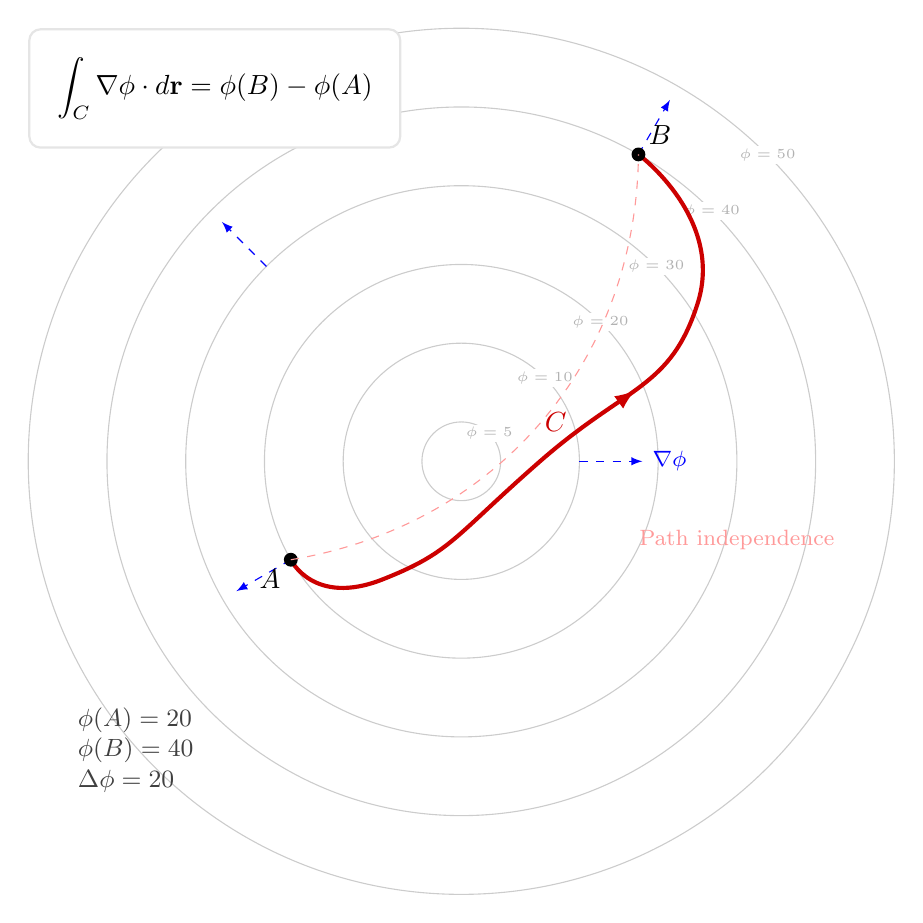
\begin{tikzpicture}[>=latex, font=\sffamily, thick]
		
		% --- 1. Draw Contour Lines (Scalar Field phi) ---
		% Simulating a potential field phi(x,y) = x^2 + y^2
		% Drawn as concentric circles (equipotential lines)
		\foreach \r/\val in {0.5/5, 1.5/10, 2.5/20, 3.5/30, 4.5/40, 5.5/50} {
			\draw[gray!40, thin] (0,0) circle (\r);
			% Add small label to some contours
			\node[gray!60, font=\tiny, fill=white, inner sep=1pt] at (45:\r) {$\phi=\val$};
		}
		
		% --- 2. Define Points A and B ---
		% A is on a lower contour, B is on a higher contour
		\coordinate (A) at (210:2.5); % On r=2.5 circle
		\coordinate (B) at (60:4.5);  % On r=4.5 circle
		
		% --- 3. Draw the Path C ---
		% An arbitrary wavy path connecting A to B
		\draw[
		red!80!black, 
		line width=1.5pt, 
		decoration={markings, mark=at position 0.6 with {\arrow{>}}},
		postaction={decorate}
		] 
		plot [smooth, tension=1] coordinates { 
			(A) 
			(-1, -1.5) 
			(1, 0) 
			(3, 2) 
			(B) 
		};
		
		% Label the path
		\node[red!80!black] at (1.2, 0.5) {$C$};
		
		% --- 4. Draw Gradient Vectors (nabla phi) ---
		% Gradient is always perpendicular to contour lines, pointing outward (uphill)
		\foreach \angle/\rad in {210/2.5, 60/4.5, 0/1.5, 135/3.5} {
			\draw[->, blue, dashed, thin] (\angle:\rad) -- (\angle:\rad+0.8);
		}
		% Label one gradient vector
		\node[blue, font=\footnotesize, right] at (0:2.3) {$\nabla \phi$};
		
		% --- 5. Draw and Label Endpoints ---
		\fill[black] (A) circle (2.5pt) node[below left] {$A$};
		\fill[black] (B) circle (2.5pt) node[above right] {$B$};
		
		% --- 6. Add Annotation for Potentials ---
		% Visualizing the "height" difference
		\node[anchor=north west, align=left, font=\small, color=gray!50!black] 
		at (-5, -3) {
			$\phi(A) = 20$\\
			$\phi(B) = 40$\\
			$\Delta \phi = 20$
		};
		
		% --- 7. The Theorem Text Box ---
		\node[
		anchor=north west, 
		fill=white, 
		draw=gray!20, 
		rounded corners, 
%		drop shadow, 
		inner sep=10pt
		] at (-5.5, 5.5) {
			$\displaystyle \int_C \nabla\phi \cdot d\mathbf{r} = \phi(B) - \phi(A)$
		};
		
		% Optional: Add a second path to imply path independence?
		% Let's keep it clean, but adding a dashed path suggests the property.
		\draw[dashed, red!40, thin] (A) to[bend right=40] (B);
		\node[red!40, font=\footnotesize] at (3.5, -1) {Path independence};
		
	\end{tikzpicture}
	
\end{document}